We use the
\href{https://statistics.laerd.com/statistical-guides/pearson-correlation-coefficient-statistical-guide.php}{Pearson
correlation coefficient} to determine the similarity between the
derivatives of the global Q function critic and the local approximations
we use a-la DDPG.

The motivation of the paper states that we wish to approximate this
global Q using less expensive local Q approximator functions. We can
ignore the magnitude and actual values of the two functions as we only
wish to examine the updates, i.e.~derivatives of these functions. Thus,
we attempt to \textbf{find a positive correlation between
\(\frac{\partial Q_{global}}{\partial t}\) and
\(\frac{\partial Q_{local}}{\partial t}\).}

\href{https://statistics.laerd.com/statistical-guides/pearson-correlation-coefficient-statistical-guide.php}{According
to statistics.laerd.com}, this table can be used to roughly understand
the importance of correlations between two functions.

\begin{figure}[h]
\centering
\begin{subfigure}{.5\textwidth}
  \centering
  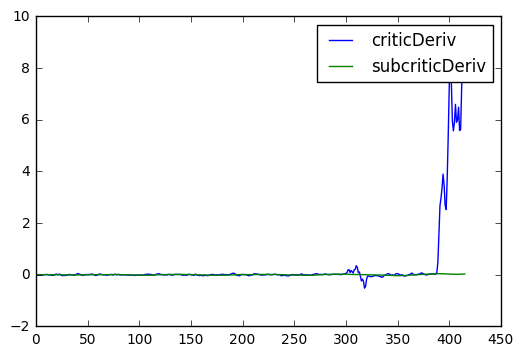
\includegraphics[width=.6\linewidth]{exp1_analysis_1_1.png}
  \caption{Critic and subcritic derivatives}
  \label{fig:sub1}
\end{subfigure}%
\begin{subfigure}{.5\textwidth}
  \centering
  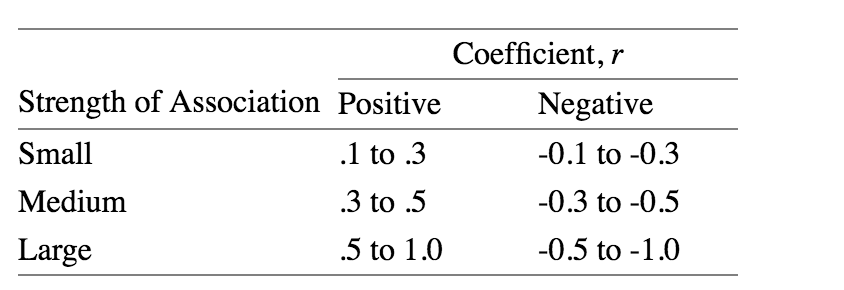
\includegraphics[width=.6\linewidth]{pearson_table.png}
  \caption{Pearson interpretation}
  \label{fig:sub2}
\end{subfigure}
\caption{Analysis figures}
\label{fig:test}
\end{figure}

In the mountain car experiment, we find a Pearson r-value of
0.389. Thus, we can infer that there is a ``weak
correlation'' between the derivatives of the global and local function.

These numbers are not necessarily significant without smoothing. As the
local approximations are inherently stochastic methods, we must apply
some smoothing techniques to obtain reasonable results.